\documentclass[a4paper,12pt]{article}

\usepackage[utf8]{inputenc}
\usepackage[left=0.5in,right=0.5in,top=1in,bottom=1in]{geometry}
\usepackage{amsmath,amssymb,amsfonts}
\usepackage{pgfplots,graphicx,calc,changepage}
\pgfplotsset{compat=newest}
\usepackage{enumitem}
\usepackage{fancyhdr}
\usepackage[colorlinks = true, linkcolor = blue]{hyperref}

% Syntax highlighting
\usepackage{listings}
\usepackage{xcolor}

\definecolor{codegreen}{rgb}{0.40,0.62,0.07}
\definecolor{codegray}{rgb}{0.5,0.5,0.5}
\definecolor{codeblue}{rgb}{0.09,0.57,0.73}
\definecolor{backcolour}{rgb}{1,1,1}

\lstdefinestyle{mystyle}{
    backgroundcolor=\color{backcolour},   
    commentstyle=\color{codegreen},
    keywordstyle=\color{magenta},
    numberstyle=\tiny\color{codegray},
    stringstyle=\color{codeblue},
    basicstyle=\ttfamily\small,
    breaklines=true,                     
    keepspaces=true,                 
    numbers=left,                    
    numbersep=5pt,                  
    showspaces=false,
    showstringspaces=false,
    showtabs=false,                  
    tabsize=4
}

\lstset{style=mystyle}

\lstdefinelanguage{Julia}%
{morekeywords={abstract,break,case,catch,const,continue,do,else,elseif,%
		end,export,false,for,function,immutable,import,importall,if,in,%
		macro,module,otherwise,quote,return,switch,true,try,type,typealias,%
		using,while},%
	sensitive=true,%
	alsoother={$},%
	morecomment=[l]\#,%
	morecomment=[n]{\#=}{=\#},%
	morestring=[s]{"}{"},%
	morestring=[m]{'}{'},%
}[keywords,comments,strings]%

\newcommand{\nats}{\mathbb{N}}
\newcommand{\reals}{\mathbb{R}}
\newcommand{\rats}{\mathbb{Q}}
\newcommand{\ints}{\mathbb{Z}}
\newcommand{\comps}{\mathbb{C}}
\newcommand{\pols}{\mathcal{P}}
\newcommand{\cants}{\Delta\!\!\!\!\Delta}
\newcommand{\eps}{\varepsilon}
\newcommand{\st}{\backepsilon}
\newcommand{\abs}[1]{\left| #1 \right|}
\newcommand{\dom}[1]{\mathrm{dom}\left(#1\right)}
\newcommand{\for}{\text{ for }}
\newcommand{\dd}{\mathrm{d}}
\newcommand{\spn}{\mathrm{sp}}
\newcommand{\nul}{\mathcal{N}}
\newcommand{\col}{\mathrm{col}}
\newcommand{\rank}{\mathrm{rank}}
\newcommand{\norm}[1]{\lVert #1 \rVert}
\newcommand{\inner}[1]{\left\langle #1 \right\rangle}
\newcommand{\pmat}[1]{\begin{pmatrix} #1 \end{pmatrix}}
\renewcommand{\and}{\text{ and }}

\newsavebox{\qed}
\newenvironment{proof}[2][$\square$]
    {\setlength{\parskip}{0pt}\par\textit{Proof:} #2\setlength{\parskip}{0.25cm}
        \savebox{\qed}{#1}
        \begin{adjustwidth}{\widthof{Proof:}}{}
    }
    {
        \hfill\usebox{\qed}\end{adjustwidth}
    }

\pagestyle{fancy}
\fancyhead{}
\lhead{Caleb Jacobs}
\chead{APPM 5610: Numerical Analysis II}
\rhead{Homework \#8}
\cfoot{}
\setlength{\headheight}{35pt}
\setlength{\parskip}{0.25cm}
\setlength{\parindent}{0pt}

\begin{document}

\textbf{Problems}
\begin{enumerate}[label = (\arabic*)]
	\item A popular explicit Runge-Kutta method is defined by the following formulas:
	\begin{align*}
		k_1 		 &= hf(x_n, y_n) \\
		k_2 		 &= hf(x_n + \frac{1}{2}h, y_n + \frac{1}{2} k_1) \\
		k_3 		 &= hf(x_n + \frac{1}{2}h, y_n + \frac{1}{2}k_2) \\
		k_4          &= hf(x_n + h, y_n + k_3) \\
		y_{n + 1} &= y_n + \frac{1}{6} (k_1 + 2k_2 + 2k_3 + k_4)
	\end{align*}
	
	With this Runge-Kutta method in mind, we want to approximate the region of absolute stability acting on the standard test problem $ y' = \lambda y $. So, let's just plug this test problem into our scheme as
	\begin{align*}
		k_1 		 &= h \lambda y_n \\
		k_2          &= h(\lambda y_n + \frac{1}{2} k_1) \\
		k_3 		 &= h(\lambda y_n + \frac{1}{2} k_2) \\
		k_4          &= h(\lambda y_n + k_3) \\
		y_{n + 1} &= y_n + \frac{1}{6} (k_1 + 2k_2 + 2k_3 + k_4) \\
						&= y_n + h \lambda y_n + \frac{1}{2} (h \lambda)^2 y_n + \frac{1}{6} (h \lambda)^3 y_n + \frac{1}{24} (h \lambda)^4 y_n \\
					    &= \left(1 + h \lambda + \frac{1}{2} (h \lambda)^2 + \frac{1}{6} (h \lambda)^3 + \frac{1}{24} (h \lambda)^4 \right) y_n.
	\end{align*}
	If we let, $ z = h \lambda $, then our final expression can be written as
	\[
		y_{n + 1} = \left(1 + z + \frac{1}{2} z^2 + \frac{1}{6} z^3 + \frac{1}{24} z^4 \right) y_n
	\]
	which shows us our scheme will converge if
	\[
		p(z) = \abs{1 + z + \frac{1}{2} z^2 + \frac{1}{6} z^3 + \frac{1}{24} z^4} < 1.
	\]
	This equation is quite tricky to work with so we will find try to approximate the region of absolute stability. First, we will find the solutions of the equation $ \abs{p(z)} = 1$ for purely real $ z $. Doing so, we find the two real roots to be at
	\[
		z = 0
	\]
	and 
	\[
		z = \frac{1}{3} \left(-10 \sqrt[3]{\frac{2}{9 \sqrt{29}-43}}+2^{2/3} \sqrt[3]{9 \sqrt{29}-43}-4\right).
	\]
	Next, we seek the purely imaginary solutions of $ p(z) = 1 $ which yields
	\[
		z = - i 2 \sqrt{2}
	\]
	and 
	\[
		z = i 2 \sqrt{2}.
	\]
	
	\newpage
	Plotting all of these points marks out the rough region below
	\begin{figure}[h!]
		\centering
		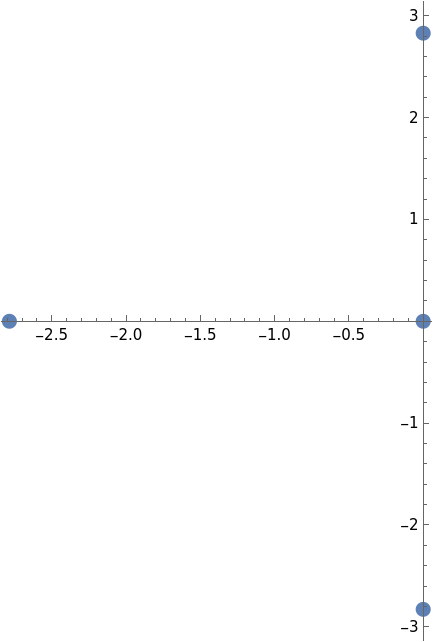
\includegraphics[width = 0.4\textwidth]{Images/Dots.png}
	\end{figure}

	We can compare this rough region with Mathematica's region plot as
	\begin{figure}[h!]
		\centering
		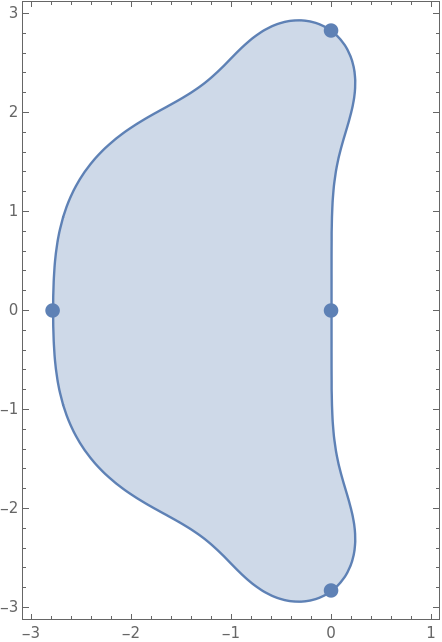
\includegraphics[width = 0.4\textwidth]{Images/True.png}
	\end{figure}

	\newpage
	\item One seeks the solution of the eigenvalue problem
	\[
		\frac{\dd}{\dd x} \left(\frac{1}{1 + x} \frac{\dd y}{\dd x}\right) + \lambda y = 0
	\]
	with boundary conditions $ y(0) = y(1) = 0 $. We want to find the $ \lambda $ such that the initial conditions $ y(0) = 0 $ and $ y'(0) = 1 $ leads to the boundary condition $ y(1) = 0 $ being met. Using my Richardson's extrapolation and trapezoidal method code from the last assignment, we can introduce the bisection method to find the desired $ \lambda $. The bisection method is super easy to implement (\emph{my code is attached at the end}), we just need to choose a starting search range. In this case, we will start with the range $ [6.7, 6.8] $. Then, because our ODE is second order, we will need to reduce the ODE into a system of first order ODEs. Reducing this ODE yields the system
	\begin{align*}
		y' &= u \\
		u' &= \frac{1}{1 + x} u - (1 + x) y
	\end{align*}
	with initial conditions $ y(0) = 0 $ and $ u(0) = 1 $. Then, plugging this system and search range into my code finds $ \lambda $ to be
	\[
		\lambda = 6.773873469310571
	\]
	which, when compared to Mathematica's solution, has a relative error of
	\[
		 1.4423 \cdot 10^{-15}.
	\]
	So, it appears my code is working well and is also quite fast!
\end{enumerate}

\textbf{Code Used}

\emph{Note: some of the symbols are missing in my code snippet because \LaTeX\ does not support all unicode characters.}

\vspace{-0.5cm}
\rule{\textwidth}{.4pt}
\lstinputlisting[language = Julia]{Code/Trapezoidal_ODE.jl}
\rule{\textwidth}{.4pt}
\end{document}